%%% Template ITA - Dissertação/Tese
%%%
%++++++++++++++++++++++++++++++++++++++++++++++++++++++++++++++++++++++++++++++
% Para alterar o TIPO DE DOCUMENTO, preencher a linha abaixo \documentclass[?]{?}
%   \documentclass[tg]{ita}			= Trabalho de Graduacao
%   \documentclass[tgfem]{ita}	= Para Engenheiras
%   								msc     		= Dissertacao de Mestrado
%   								mscfem   		= Para Mestras
%   								dsc      		= Tese de Doutorado
%   								dscfem   		= Para Doutoras
%   								quali    		= Exame de Qualificacao
%   								qualifem 		= Exame de Qualificacao para Doutoras
% Para 'Draft Version'/'Versao Preliminar' com data no rodape, adicionar 'dv':
%   \documentclass[dsc, dv]{ita}
% Para trabalhos em Inglês, adicionar 'eng':
%   \documentclass[dsc, eng]{ita}
%		\documentclass[dsc, eng, dv]{ita}
%++++++++++++++++++++++++++++++++++++++++++++++++++++++++++++++++++++++++++++++
\documentclass[msc]{ita}    % ITA.cls based on standard book.cls
% Quando alterar a classe, por exemplo de [msc] para [msc, eng]) rode mais uma vez o botão BUILD OUTPUT caso haja erro

% Comando para marcar campos a preencher (remover \placeholder ao preencher)
\definecolor{PHREDD}{rgb}{1,0,0}
\newcommand{\placeholder}[1]{{\color{PHREDD}#1}}

% Comando para exibir fullcite alinhado à esquerda (como nas referências)
\newcommand{\fullciteblock}[1]{%
  \begin{flushleft}
    \fullcite{#1}
  \end{flushleft}
}

% Código do tipo de documento para a Folha de Registro (DM, TG, TD)
\newcommand{\itadoccode}{%
  \ifdefstring{\itaoptionlevel}{msc}{DM}{%
  \ifdefstring{\itaoptionlevel}{mscfem}{DM}{%
  \ifdefstring{\itaoptionlevel}{tg}{TG}{%
  \ifdefstring{\itaoptionlevel}{tgfem}{TG}{%
  \ifdefstring{\itaoptionlevel}{dsc}{TD}{%
  \ifdefstring{\itaoptionlevel}{dscfem}{TD}{%
  \ifdefstring{\itaoptionlevel}{quali}{TD}{%
  \ifdefstring{\itaoptionlevel}{qualifem}{TD}{XX}}}}}}}}%
}

\usepackage{textcomp}    % símbolos e melhor cópia/colagem no PDF
\usepackage{sourcecodepro} % fonte monoespaçada Adobe (substitui CM Typewriter)
\usepackage{graphicx}
\usepackage{epsfig}
\usepackage{amsmath}
\usepackage{amssymb}
\usepackage{subfig}
\usepackage{multirow}
\usepackage{float}
\usepackage{amsthm}
\usepackage{url}         % formats URL addresses properly
\renewcommand{\UrlFont}{\ttfamily\footnotesize} % URL em tamanho menor
\usepackage{tikz}
\usetikzlibrary{arrows.meta,calc,shapes.geometric,positioning}
\usepackage{pgfplots}
\pgfplotsset{compat=1.18}

% Compatibilidade: algumas entradas ABNT podem usar \htmladdnormallink
\providecommand{\htmladdnormallink}[2]{\href{#2}{#1}}
\providecommand{\htmladdnormallinkfoot}[2]{\href{#2}{#1}}

\usepackage{appendix}    % allows appendix section to be included
\usepackage{lscape}      % allows a page to be rendered in landscape mode
\usepackage{multicol}    % allows text in multi columns
\usepackage{cancel}      % needed to show canceled terms in equations
\usepackage{lettrine}
\usepackage{float}
\usepackage{placeins}

% Better verbatim
\usepackage{fancyvrb}
\usepackage{fvextra}

% csquotes must be loaded after fvextra to avoid lineno warning
\usepackage{csquotes}
\MakeOuterQuote{"}  % Converte "texto" em aspas tipográficas

% Better abnt
% backend=biber
% style=abnt: Carrega as normas da ABNT (NBR 6023)
\usepackage[backend=biber, style=abnt, backref=true, giveninits=true]{biblatex}

% Coloca "apud" em itálico - redefine a macro diretamente
\AtBeginDocument{%
  \renewcommand{\addapud}{%
    \renewcommand*{\compcitedelim}{%
      \ifnumequal{\value{multicitecount}}{\value{multicitetotal}}%
        {\space\textit{apud}}%
        {\addsemicolon}%
      \space}%
    \renewcommand*{\multicitedelim}{%
      \ifnumequal{\value{multicitecount}}{\value{multicitetotal}}%
        {\space\textit{apud}}%
        {\addsemicolon}%
      \space}%
    \renewcommand*{\textcitedelim}{%
      \ifnumequal{\value{multicitecount}}{\value{multicitetotal}}%
        {\addspace\textit{apud}}%
        {\addsemicolon}%
      \space}%
  }%
}

% Redefine macro booktitle: usa titlecase para inproceedings, comportamento original para outros
\renewbibmacro*{booktitle}{%
  \ifboolexpr{%
    test {\iffieldundef{booktitle}}%
    and%
    test {\iffieldundef{booksubtitle}}%
  }%
    {}%
    {\printtext[booktitle]{%
      \ifentrytype{inproceedings}%
        {\printfield[titlecase]{booktitle}\normalfont{ [\ldots].}}%  % inproceedings: titlecase + [...].
        {\usebibmacro{booktitleiskey}{%       % outros: comportamento ABNT original
          \printfield[upperfirst]{booktitle}%
        }{%
          \printfield[titlecase]{booktitle}%
        }}%
      \iffieldendswithpunct{booktitle}{%
        \normalfont{\setunit*{\addspace}}%
      }{%
        \normalfont{\setunit*{\subtitlepunct}}%
      }%
      \printfield[normalfont]{booksubtitle}}%
    \newunit}%
  \printfield{booktitleaddon}%
}
% =============================================================================
% Campos customizados para patentes ABNT (NBR 6023:2018)
% Ordem: Inventor. Título. Depositante. Procurador. Número. Depósito. Concessão.
% =============================================================================
% Mapeamento: nomes amigáveis → campos internos
\DeclareSourcemap{
  \maps[datatype=bibtex]{
    \map{
      \pertype{patent}
      \step[fieldsource=depositante, fieldtarget=usera]
      \step[fieldsource=procurador, fieldtarget=userb]
      \step[fieldsource=deposito, fieldtarget=userc]
      \step[fieldsource=concessao, fieldtarget=userd]
    }
  }
}
% Formatos de saída
\DeclareFieldFormat[patent]{usera}{Depositante\addcolon\addspace #1}
\DeclareFieldFormat[patent]{userb}{Procurador\addcolon\addspace #1}
\DeclareFieldFormat[patent]{userc}{Depósito\addcolon\addspace #1}
\DeclareFieldFormat[patent]{userd}{Concessão\addcolon\addspace #1}

% Redefine driver de patente para ordem ABNT
\DeclareBibliographyDriver{patent}{%
  \usebibmacro{bibindex}%
  \usebibmacro{begentry}%
  \usebibmacro{author/editor+others}%
  \setunit{\labelnamepunct}%
  \usebibmacro{title}%
  \setunit{\addperiod\addspace}%
  \printfield{usera}%
  \setunit{\addperiod\addspace}%
  \printfield{userb}%
  \setunit{\addperiod\addspace}%
  \printfield{number}%
  \setunit{\addperiod\addspace}%
  \printfield{userc}%
  \setunit{\addperiod\addspace}%
  \printfield{userd}%
  \setunit{\addperiod\addspace}%
  \usebibmacro{doi+eprint+url}%
  \usebibmacro{finentry}%
}

% Adicione seu arquivo .bib
\addbibresource{Referencias/referencias.bib}




% Listas conforme ABNT NBR 6024
\usepackage{enumitem}
\setlist[enumerate,1]{label=\alph*)}  % alíneas: a) b) c)
\setlist[enumerate,2]{label=--}       % subalíneas: travessão
\setlist[itemize]{label=--}           % itemize também usa travessão

\usepackage{booktabs}

% Acrônimos automáticos com backref de páginas
\usepackage{acro}
\acsetup{
  pages/display = all,
  pages/fill = {.\dotfill},
  list/heading = chapter*,
  list/name = Lista de Abreviaturas,
}
% Definições de acrônimos para o pacote acro
% Uso no texto: \ac{CTq} (primeira vez expande), \acs{CTq} (só sigla), \acl{CTq} (só longo)

\DeclareAcronym{ITA}{
  short = ITA,
  long  = Instituto Tecnológico de Aeronáutica,
}
\DeclareAcronym{ABNT}{
  short = ABNT,
  long  = Associação Brasileira de Normas Técnicas,
}
\DeclareAcronym{CTq}{
  short = CTq,
  long  = computed torque,
}
\DeclareAcronym{DC}{
  short = DC,
  long  = direct current,
}
\DeclareAcronym{EAR}{
  short = EAR,
  long  = Equação Algébrica de Riccati,
}
\DeclareAcronym{CLI}{
  short = CLI,
  long  = \textit{command-line interface},
}
\DeclareAcronym{FOSS}{
  short = FOSS,
  long  = \textit{free and open-source software},
}
\DeclareAcronym{GDL}{
  short = GDL,
  long  = graus de liberdade,
}
\DeclareAcronym{GUI}{
  short = GUI,
  long  = \textit{graphical user interface},
}
\DeclareAcronym{ISR}{
  short = ISR,
  long  = interrupção de serviço e rotina,
}
\DeclareAcronym{LMI}{
  short = LMI,
  long  = linear matrices inequalities,
}
\DeclareAcronym{MIMO}{
  short = MIMO,
  long  = multiple input multiple output,
}
\DeclareAcronym{OCR}{
  short = OCR,
  long  = \textit{optical character recognition},
}
\DeclareAcronym{PD}{
  short = PD,
  long  = proporcional derivativo,
}
\DeclareAcronym{PID}{
  short = PID,
  long  = proporcional integrativo derivativo,
}
\DeclareAcronym{PTP}{
  short = PTP,
  long  = point to point,
}
\DeclareAcronym{UARMII}{
  short = UARMII,
  long  = Underactuated Robot Manipulator II,
}
\DeclareAcronym{VSC}{
  short = VSC,
  long  = variable structure control,
}


%++++++++++++++++++++++++++++++++++++++++++++++++++++++++++++++++++++++++++++++
% Espaçamento padrão de todo o documento
%++++++++++++++++++++++++++++++++++++++++++++++++++++++++++++++++++++++++++++++
\onehalfspacing

%singlespacing Para um espaçamento simples
%onehalfspacing Para um espaçamento de 1,5
%doublespacing Para um espaçamento duplo

%++++++++++++++++++++++++++++++++++++++++++++++++++++++++++++++++++++++++++++++
% Identificacoes (se o trabalho for em inglês, insira os dados em inglês)
% Para entradas abreviadas de Professora (Profa.) em português escreva: Prof$^\textnormal{a}$.
%++++++++++++++++++++++++++++++++++++++++++++++++++++++++++++++++++++++++++++++
\course{\placeholder{Engenharia Aeronáutica e Mecânica}}  % Programa de PG ou Curso de Graduação
\area{\placeholder{Área de Concentração}} % Área de concentração na PG (Não utilizado no caso de TG)

% Autor do trabalho: Nome Sobrenome
\authorgender{masc}                     %sexo: masc ou fem
\author{Nome}{Sobrenome}
\itaauthoraddress{\placeholder{Rua, número}}{\placeholder{CEP}}{São José dos Campos--SP}

% Titulo da Tese/Dissertação
\title{Título do Trabalho}

% Orientador
\advisorgender{masc}                    % masc ou fem
\advisor{Prof.~Dr.}{\placeholder{Nome do Orientador}}{ITA}

% Coorientador (Caso não haja coorientador, colocar ambas as variáveis \coadvisorgender e \coadvisor comentadas, com um % na frente)
\coadvisorgender{fem}									% masc ou fem
\coadvisor[Coorientadora]{Prof$^\textnormal{a}$.~Dr$^\textnormal{a}$.}{\placeholder{Nome da Coorientadora}}{ITA}

% Pró-reitor da Pós-graduação (opcional - comentar para não aparecer na folha de rosto)
% \bossgender{masc}												% masc ou fem
% \boss{Prof.~Dr.}{\placeholder{Nome do Pró-Reitor}}

%Coordenador do curso no caso de TG
\bosscoursegender{masc}									% masc ou fem
\bosscourse{Prof.~Dr.}{\placeholder{Nome do Coordenador}}

% Palavras-Chaves informadas pela Biblioteca -> utilizada na CIP
\kwcip{\placeholder{Palavra-chave 1}}
\kwcip{\placeholder{Palavra-chave 2}}
\kwcip{\placeholder{Palavra-chave 3}}

% membros da banca examinadora

\examiner{Prof. Dr.}{\placeholder{Membro da Banca 1}}{Presidente}{ITA}
\examiner{Prof. Dr.}{\placeholder{Membro da Banca 2}}{}{\placeholder{Instituição}}
\examiner{Prof. Dr.}{\placeholder{Membro da Banca 3}}{}{\placeholder{Instituição}}
% \examiner{Prof. Dr.}{\placeholder{Membro da Banca 4}}{}{\placeholder{Instituição}}
% \examiner{Prof. Dr.}{\placeholder{Membro da Banca 5}}{}{\placeholder{Instituição}}

% Data da defesa: \date{dia}{mês}{ano}
% Mês em maiúsculo se trabalho em inglês (March), minúsculo se português (março)
% Exemplo: \date{15}{março}{2026}
\date{\placeholder{dia}}{\placeholder{mês}}{\placeholder{ano}}

% Número CDU - (somente para TG)
\cdu{???.??}

% Glossario
%\makeglossary
\frontmatter

\begin{document}
% Folha de Rosto e Capa para o caso do TG
\maketitle

% Dedicatoria: Nao esqueca essa secao  ... :-)
\begin{itadedication}
\placeholder{Dedico este trabalho a minha família, amigos e todos que me apoiaram nesta jornada.}
\end{itadedication}

% Agradecimentos
\begin{itathanks}
\placeholder{Agradeço ao meu orientador, Prof. Dr. Nome do Orientador, pela orientação e confiança depositada na realização deste trabalho.}

\placeholder{Agradeço também aos professores do ITA pelos ensinamentos e à minha família pelo apoio incondicional.}

\placeholder{Por fim, agradeço aos colegas de laboratório e a todos que contribuíram direta ou indiretamente para a conclusão deste trabalho.}

\end{itathanks}

% Epígrafe
\thispagestyle{empty}
\ifhyperref\pdfbookmark[0]{\nameepigraphe}{epigrafe}\fi
\begin{flushright}
\begin{spacing}{1}
\mbox{}\vfill
{\sffamily\itshape
"Na natureza nada se cria, nada se perde, tudo se transforma."}\\
--- \textsc{Antoine Lavoisier}

\end{spacing}
\end{flushright}

% Resumo
\begin{abstract}
\noindent
\placeholder{Inserir aqui o resumo em português. O resumo deve apresentar de forma concisa o objetivo, a metodologia, os resultados e as conclusões do trabalho. Deve ser redigido em parágrafo único, sem recuo na primeira linha, com espaçamento simples entre linhas. O resumo não deve ultrapassar 500 palavras para dissertações e teses, ou 250 palavras para trabalhos de graduação.}

\end{abstract}

% Abstract
\begin{englishabstract}
\noindent
\placeholder{Insert the abstract in English here. The abstract should concisely present the objective, methodology, results, and conclusions of the work. It should be written in a single paragraph, without indentation on the first line, with single line spacing. The abstract should not exceed 500 words for dissertations and theses, or 250 words for undergraduate works.}

\end{englishabstract}

% Lista de figuras
\listoffigures %opcional

% Lista de tabelas
\listoftables %opcional

% Lista de abreviaturas (automática com acro)
\printacronyms

% Lista de simbolos
\listofsymbols
\input{PreTextuais/listasimbolos} %opcional

% Sumario
\tableofcontents


\mainmatter
% Os capitulos comecam aqui

\chapter{Introdução}
Após anos de dedicação ao curso, o aluno se depara com o desafio de confeccionar sua dissertação ou tese. Este documento visa orientar esse processo, esclarecendo as normas e boas práticas para a produção de trabalhos acadêmicos no \ac{ITA}.

Os modelos de trabalhos acadêmicos do \ac{ITA} seguem as normas da \ac{ABNT}, em especial a NBR 14724 (trabalhos acadêmicos) e a NBR 6023 (referências bibliográficas). Embora tais normas utilizem terminologia específica da área de documentação, este template busca simplificar sua aplicação através de formatação automatizada.

\section{Por que \LaTeX?}

O \LaTeX{} é um sistema de preparação de documentos amplamente utilizado na comunidade acadêmica e científica. Suas principais vantagens incluem:

\begin{enumerate}
    \item Qualidade tipográfica superior, especialmente para expressões matemáticas como $\int_0^\infty e^{-x^2} dx = \frac{\sqrt{\pi}}{2}$;
    \item Gerenciamento automático de referências cruzadas, numeração de figuras, tabelas e equações;
    \item Formatação consistente em todo o documento;
    \item Separação entre conteúdo e apresentação, permitindo que o autor foque no texto;
    \item Controle de versão facilitado por ser baseado em texto puro; e
    \item Ampla disponibilidade de pacotes para necessidades específicas.
\end{enumerate}

Este template utiliza o sistema Bib\LaTeX{} com \textit{backend} Biber para gerenciamento de referências bibliográficas, garantindo conformidade com as normas ABNT vigentes e oferecendo recursos avançados como \textit{backref} (indicação das páginas onde cada referência é citada).

\section{Tipos de Trabalhos Acadêmicos}

Este template atende aos seguintes tipos de trabalhos acadêmicos do \ac{ITA}:

\begin{enumerate}
    \item Trabalho de Graduação, para obtenção do diploma de Engenheiro;
    \item Dissertação de Mestrado, para obtenção do título de Mestre em Ciências;
    \item Dissertação de Mestrado Profissional, para obtenção do título de Mestre; e
    \item Tese de Doutorado, para obtenção do título de Doutor em Ciências.
\end{enumerate}

A configuração do tipo de documento é feita através das opções da classe, como \texttt{msc} para mestrado, \texttt{dsc} para doutorado, ou \texttt{tg} para trabalho de graduação.

\section{Estrutura do Documento}

A apresentação do texto deve obedecer à ordem dos elementos descritos na Tabela~\ref{tab:ordem-apresentacao}, conforme a ABNT NBR 14724.

\begin{table}[htbp]
\centering
\caption{Ordem de apresentação da Dissertação ou Tese.}
\label{tab:ordem-apresentacao}
\begin{tabular}{p{2.5cm}p{7.3cm}p{2.2cm}p{2.2cm}}
\toprule
Elemento & Estrutura (sequencial) & Versão preliminar & Versão final \\
\midrule
\multirow{15}{*}{Pré-textuais} & Capa & obrigatório & obrigatório \\
 & Folha de rosto & obrigatório & obrigatório \\
 & Verso da folha de rosto & não colocar & obrigatório \\
 & Folha da banca & obrigatório & obrigatório \\
 & Dedicatória & opcional & opcional \\
 & Agradecimentos & opcional & opcional \\
 & Epígrafe & opcional & opcional \\
 & Resumo & obrigatório & obrigatório \\
 & Abstract & obrigatório & obrigatório \\
 & Lista de Figuras & opcional & opcional \\
 & Lista de Tabelas & opcional & opcional \\
 & Lista de Abreviaturas e Siglas & opcional & opcional \\
 & Lista de Símbolos & opcional & opcional \\
 & Sumário & obrigatório & obrigatório \\
\midrule
\multirow{3}{*}{Textuais} & Introdução & obrigatório & obrigatório \\
 & Desenvolvimento & obrigatório & obrigatório \\
 & Conclusão & obrigatório & obrigatório \\
\midrule
\multirow{5}{*}{Pós-textuais} & Referências & obrigatório & obrigatório \\
 & Apêndice(s) & opcional & opcional \\
 & Anexo(s) & opcional & opcional \\
 & Glossário & opcional & opcional \\
 & Folha de Registro do Documento & não colocar & obrigatório \\
\bottomrule
\end{tabular}
\end{table}

Ao contrário da versão preliminar, na versão final devem ser incorporados os elementos ``Verso da folha de rosto'' e ``Folha de Registro do Documento''. A ``Folha de Registro do Documento'' não é um item da ABNT e sim um documento necessário para atender a NPA-ITA-011B:2023.

Tanto o Resumo quanto o Abstract são itens obrigatórios, independentemente se o texto seja escrito em português ou inglês.

\section{Estrutura da Introdução}

A introdução de uma dissertação ou tese deve conter os seguintes elementos:

\begin{enumerate}
    \item contextualização do tema e motivação para o estudo;
    \item revisão bibliográfica sucinta, situando o trabalho no estado da arte;
    \item definição clara dos objetivos (geral e específicos);
    \item no caso de doutorado, descrição das contribuições originais; e
    \item descrição da metodologia e organização dos capítulos.
\end{enumerate}

\section{Organização deste Documento}

Este documento está organizado da seguinte forma:

O Capítulo 2 apresenta orientações sobre revisão bibliográfica e demonstra o uso de citações e figuras.

O Capítulo 3 exemplifica um capítulo de Metodologia, comum em dissertações e teses.

O Capítulo 4 aborda aspectos de formatação, incluindo margens, fontes, espaçamento e paginação conforme as normas ABNT.

O Capítulo 5 trata da elaboração de citações e referências bibliográficas, demonstrando os diversos tipos de fontes e suas formatações.

O Capítulo 6 orienta sobre a confecção da versão final em mídia digital para depósito na biblioteca.

O Capítulo 7 explica o preenchimento da Folha de Registro do Documento.

O Capítulo 8 apresenta as considerações finais.


\chapter{Revisão Bibliográfica}
A revisão bibliográfica, também chamada de revisão da literatura ou fundamentação teórica, é uma etapa fundamental de qualquer trabalho acadêmico. Seu objetivo é situar a pesquisa no contexto do conhecimento existente, identificando lacunas, tendências e contribuições anteriores.

\section{Propósito da Revisão Bibliográfica}

A revisão bibliográfica cumpre múltiplos propósitos:

\begin{enumerate}
    \item demonstrar domínio sobre o tema de pesquisa;
    \item identificar o estado da arte e as lacunas existentes;
    \item justificar a relevância e originalidade do trabalho;
    \item estabelecer a base teórica para a metodologia adotada; e
    \item evitar duplicação de esforços já realizados.
\end{enumerate}

Recomenda-se que a revisão seja organizada por temas ou conceitos, e não simplesmente por ordem cronológica de publicação. Cada trabalho citado deve ser analisado criticamente, destacando suas contribuições e limitações.

\section{Normas ABNT para Trabalhos Acadêmicos}

A elaboração de dissertações e teses no Brasil é regida por um conjunto de normas da \ac{ABNT}. As principais são:

\begin{enumerate}
    \item NBR 14724 -- Trabalhos acadêmicos: apresentação;
    \item NBR 6023 -- Referências: elaboração;
    \item NBR 10520 -- Citações em documentos;
    \item NBR 6024 -- Numeração progressiva das seções;
    \item NBR 6027 -- Sumário: apresentação;
    \item NBR 6028 -- Resumo: apresentação; e
    \item NBR 6034 -- Índice: apresentação.
\end{enumerate}

Este template implementa automaticamente a maioria dessas normas através da classe \texttt{ita.cls} e do pacote Bib\LaTeX{} com estilo ABNT.

\section{Tipos de Citação}

O sistema Bib\LaTeX{} com estilo ABNT oferece diversos comandos para citação. A seguir, demonstramos os principais tipos.

\subsection{Citação Indireta}

A citação indireta ocorre quando parafraseamos as ideias de um autor. Utiliza-se o comando \texttt{\textbackslash cite\{\}}:

\begin{itemize}
    \item Segundo a literatura, sistemas de controle robusto são essenciais para aplicações críticas \cite{Sbornian2004}.
    \item Diversos autores trataram do tema \cite{Sbornian2004, Joea2003}.
\end{itemize}

\subsection{Citação com Autor no Texto}

Quando o nome do autor faz parte da sentença, utiliza-se \texttt{\textbackslash textcite\{\}}:

\begin{itemize}
    \item \textcite{Nascimento1970} apresentou os fundamentos teóricos do problema.
    \item Conforme demonstrado por \textcite{Sbornian2004}, a abordagem é viável.
\end{itemize}

\subsection{Citação Direta}

Citações diretas curtas (até 3 linhas) são inseridas no texto entre aspas. Para citações longas, utiliza-se o ambiente \texttt{quote} ou \texttt{citacao}:

\begin{quote}
``A formatação adequada de um trabalho acadêmico contribui para sua clareza e credibilidade, facilitando a comunicação científica.''
\end{quote}

\section{Elementos de Apoio}

A revisão bibliográfica frequentemente utiliza tabelas e equações para sintetizar informações. A Tabela \ref{tab:exemplo} demonstra a formatação adequada.

\begin{table}[ht]
\caption{Comparativo entre abordagens metodológicas}
\label{tab:exemplo}
\centering
\begin{tabular}{lccc}
    \hline
    Abordagem & Complexidade & Precisão & Custo \\
    \hline
    Analítica & Baixa & Alta & Baixo \\
    Numérica & Média & Média & Médio \\
    Experimental & Alta & Variável & Alto \\
    \hline
\end{tabular}
\end{table}

Equações também são frequentes em revisões de áreas técnicas. Por exemplo, a equação de Lagrange é fundamental em mecânica analítica:

\begin{equation} \label{eq:lagrange}
\frac{d}{dt}\left(\frac{\partial L}{\partial \dot{q}}\right) - \frac{\partial L}{\partial q} = \tau
\end{equation}

\noindent onde $L = T - V$ representa o Lagrangiano do sistema, $T$ a energia cinética, $V$ a energia potencial, $q$ as coordenadas generalizadas e $\tau$ as forças generalizadas.

\section{Figuras Vetoriais com PGFPlots}

O pacote PGFPlots permite criar gráficos de alta qualidade diretamente em \LaTeX{}, com vantagens significativas sobre imagens externas:

\begin{enumerate}
    \item qualidade vetorial (sem pixelização em qualquer escala);
    \item consistência tipográfica (mesma fonte do documento);
    \item facilidade de edição (dados no próprio código); e
    \item arquivos leves e versionáveis.
\end{enumerate}

A Figura \ref{fig:linha} apresenta um exemplo de gráfico de linhas comparando dados experimentais com modelo teórico.

\begin{figure}[ht]
\centering
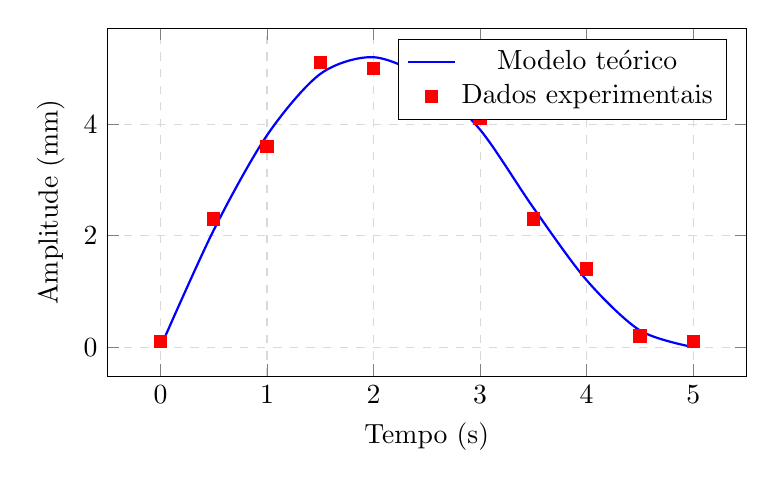
\begin{tikzpicture}
\begin{axis}[
    width=0.8\textwidth,
    height=6cm,
    xlabel={Tempo (s)},
    ylabel={Amplitude (mm)},
    legend pos=north east,
    grid=major,
    grid style={dashed,gray!30},
]
\addplot[blue, thick, mark=none, smooth] coordinates {
    (0,0) (0.5,2.1) (1,3.8) (1.5,4.9) (2,5.2) (2.5,4.8) (3,3.9) (3.5,2.5) (4,1.2) (4.5,0.3) (5,0)
};
\addlegendentry{Modelo teórico}

\addplot[red, thick, only marks, mark=square*] coordinates {
    (0,0.1) (0.5,2.3) (1,3.6) (1.5,5.1) (2,5.0) (2.5,4.6) (3,4.1) (3.5,2.3) (4,1.4) (4.5,0.2) (5,0.1)
};
\addlegendentry{Dados experimentais}
\end{axis}
\end{tikzpicture}
\caption{Comparação entre modelo teórico e dados experimentais.}
\label{fig:linha}
\end{figure}

Para comparações categóricas, gráficos de barras são frequentemente utilizados, como ilustrado na Figura \ref{fig:barras}.

\begin{figure}[ht]
\centering
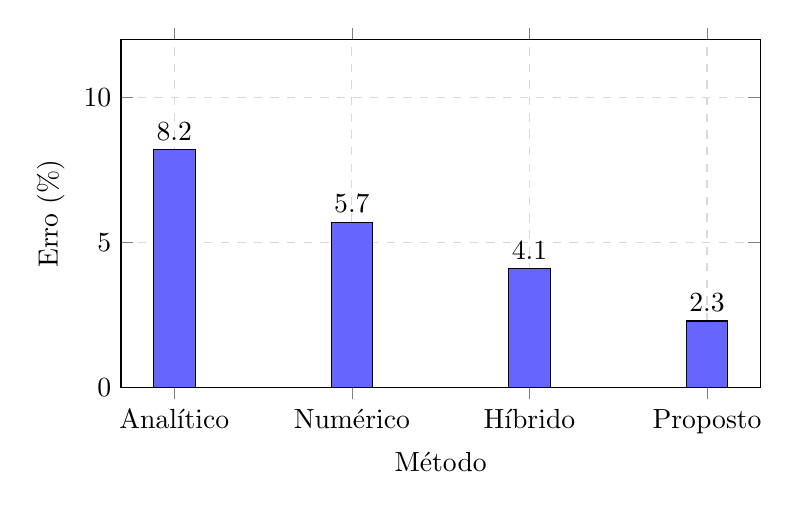
\begin{tikzpicture}
\begin{axis}[
    width=0.8\textwidth,
    height=6cm,
    ybar,
    bar width=15pt,
    xlabel={Método},
    ylabel={Erro (\%)},
    symbolic x coords={Analítico, Numérico, Híbrido, Proposto},
    xtick=data,
    nodes near coords,
    nodes near coords align={vertical},
    ymin=0,
    ymax=12,
    grid=major,
    grid style={dashed,gray!30},
    ymajorgrids=true,
]
\addplot[fill=blue!60] coordinates {
    (Analítico,8.2) (Numérico,5.7) (Híbrido,4.1) (Proposto,2.3)
};
\end{axis}
\end{tikzpicture}
\caption{Comparativo de erro entre diferentes métodos.}
\label{fig:barras}
\end{figure}

\section{Boas Práticas}

Ao redigir a revisão bibliográfica, recomenda-se:

\begin{enumerate}
    \item utilizar fontes primárias sempre que possível;
    \item priorizar publicações recentes e de periódicos com revisão por pares;
    \item manter consistência na forma de citação ao longo do texto;
    \item evitar citações excessivas em uma única sentença; e
    \item conectar os trabalhos citados com a proposta da pesquisa.
\end{enumerate}


\chapter{Metodologia}
Este capítulo descreve os materiais, equipamentos e procedimentos utilizados no desenvolvimento do trabalho. A metodologia deve ser descrita com detalhes suficientes para permitir a reprodução do estudo por outros pesquisadores.

\section{Materiais}

A descrição dos materiais deve incluir especificações técnicas, fabricantes e, quando relevante, número de lote ou pureza. A Tabela~\ref{tab:materiais} apresenta um exemplo de organização dessas informações.

\begin{table}[ht]
\centering
\caption{Materiais utilizados no experimento.}
\label{tab:materiais}
\begin{tabular}{llll}
\toprule
Material & Especificação & Fabricante & Pureza \\
\midrule
Alumínio 6061-T6 & Barra $\varnothing 25 \times 100$ mm & Alcoa & -- \\
Aço AISI 304 & Chapa 2 mm & Gerdau & -- \\
Acetona & P.A. & Sigma-Aldrich & 99,5\% \\
Resina epóxi & Araldite LY 1564 & Huntsman & -- \\
\bottomrule
\end{tabular}
\end{table}

\section{Equipamentos}

Os equipamentos devem ser descritos com modelo, fabricante e características relevantes para o experimento. Quando aplicável, incluir informações sobre calibração e incerteza de medição.

\begin{enumerate}
    \item Máquina universal de ensaios Instron 5569, capacidade 50 kN, resolução 0,1 N;
    \item Termopar tipo K, faixa $-200$ a $1260\,^{\circ}$C, incerteza $\pm 2,2\,^{\circ}$C;
    \item Balança analítica Shimadzu AUW220D, resolução 0,01 mg; e
    \item Microscópio eletrônico de varredura JEOL JSM-6010LA.
\end{enumerate}

\section{Procedimento Experimental}

O procedimento deve ser descrito de forma clara e sequencial. Fluxogramas são úteis para visualizar as etapas do processo, como ilustrado na Figura~\ref{fig:fluxograma}.

\begin{figure}[ht]
\centering
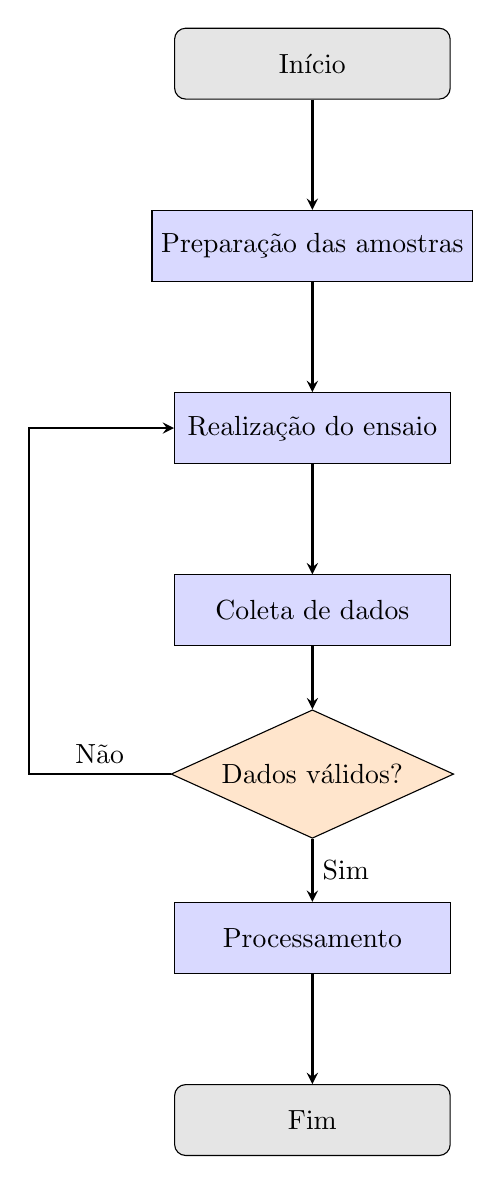
\begin{tikzpicture}[
    node distance=1.4cm,
    startstop/.style={rectangle, rounded corners, minimum width=3.5cm, minimum height=0.9cm, text centered, draw=black, fill=gray!20},
    process/.style={rectangle, minimum width=3.5cm, minimum height=0.9cm, text centered, draw=black, fill=blue!15},
    decision/.style={diamond, minimum width=2.8cm, minimum height=0.9cm, text centered, draw=black, fill=orange!20, aspect=2.2},
    arrow/.style={thick,->,>=stealth}
]
    \node (start) [startstop] {Início};
    \node (prep) [process, below=of start] {Preparação das amostras};
    \node (ensaio) [process, below=of prep] {Realização do ensaio};
    \node (coleta) [process, below=of ensaio] {Coleta de dados};
    \node (analise) [decision, below=0.8cm of coleta] {Dados válidos?};
    \node (proc) [process, below=0.8cm of analise] {Processamento};
    \node (end) [startstop, below=of proc] {Fim};

    \draw [arrow] (start) -- (prep);
    \draw [arrow] (prep) -- (ensaio);
    \draw [arrow] (ensaio) -- (coleta);
    \draw [arrow] (coleta) -- (analise);
    \draw [arrow] (analise.south) -- node[right] {Sim} (proc.north);
    \draw [arrow] (analise.west) -- ++(-1.8,0) node[above, pos=0.5] {Não} |- (ensaio.west);
    \draw [arrow] (proc) -- (end);
\end{tikzpicture}
\caption{Fluxograma do procedimento experimental.}
\label{fig:fluxograma}
\end{figure}

\subsection{Preparação das Amostras}

Descrever o processo de preparação, incluindo:
\begin{enumerate}
    \item dimensões e geometria dos corpos de prova;
    \item processos de usinagem ou conformação;
    \item tratamentos térmicos ou superficiais; e
    \item condições de armazenamento.
\end{enumerate}

\subsection{Condições de Ensaio}

As condições ambientais e parâmetros de ensaio devem ser documentados:
\begin{itemize}
    \item Temperatura ambiente: $(23 \pm 2)\,^{\circ}$C
    \item Umidade relativa: $(50 \pm 10)$\%
    \item Velocidade de carregamento: 1 mm/min
    \item Taxa de aquisição: 10 Hz
\end{itemize}

\section{Ferramentas Computacionais}

O software utilizado para análise e simulação deve ser documentado, incluindo versão e configurações relevantes. A Tabela~\ref{tab:software} apresenta as ferramentas utilizadas neste trabalho.

\begin{table}[ht]
\centering
\caption{Ferramentas computacionais utilizadas.}
\label{tab:software}
\begin{tabular}{lll}
\toprule
Ferramenta & Versão & Aplicação \\
\midrule
MATLAB & R2024a & Processamento de sinais \\
ANSYS Mechanical & 2024 R1 & Análise por elementos finitos \\
Python & 3.12 & Scripts de automação \\
\LaTeX{} & TeX Live 2024 & Redação do documento \\
\bottomrule
\end{tabular}
\end{table}

\section{Tratamento Estatístico}

Quando aplicável, descrever os métodos estatísticos utilizados para análise dos dados:

\begin{enumerate}
    \item número de repetições por condição experimental;
    \item testes estatísticos aplicados (ANOVA, teste t, etc.);
    \item nível de significância adotado; e
    \item software utilizado para análise estatística.
\end{enumerate}

Os resultados são tipicamente expressos como média $\pm$ desvio padrão ou com intervalo de confiança de 95\%.

% \chapter{Controle Robusto de Concretos Caóticos}
% \input{Cap3/cap3_old}
\chapter{Resultados}
Este capítulo apresenta os resultados obtidos a partir da metodologia descrita no Capítulo 3. Os dados são organizados em tabelas e gráficos para facilitar a análise e comparação com valores teóricos ou da literatura.

\section{Resultados Experimentais}

A Tabela~\ref{tab:resultados} apresenta os valores medidos para cada condição de ensaio, incluindo a incerteza associada.

\begin{table}[H]
\centering
\caption{Resultados dos ensaios de tração.}
\label{tab:resultados}
\begin{tabular}{lccc}
\toprule
Amostra & Tensão máxima (MPa) & Deformação (\%) & Módulo (GPa) \\
\midrule
A1 & $285 \pm 12$ & $18,2 \pm 0,8$ & $71,3 \pm 1,5$ \\
A2 & $291 \pm 10$ & $17,8 \pm 0,6$ & $72,1 \pm 1,2$ \\
A3 & $278 \pm 15$ & $19,1 \pm 1,0$ & $70,8 \pm 1,8$ \\
\midrule
Média & $285 \pm 7$ & $18,4 \pm 0,5$ & $71,4 \pm 0,9$ \\
\bottomrule
\end{tabular}
\end{table}

\section{Análise Gráfica}

A Figura~\ref{fig:resultados} compara os valores experimentais com os valores teóricos previstos pelo modelo.

\begin{figure}[H]
\centering
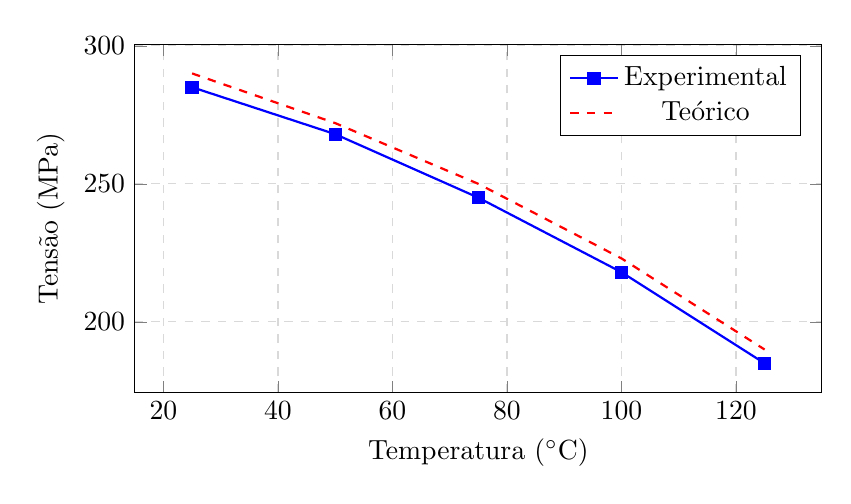
\begin{tikzpicture}
\begin{axis}[
    width=0.85\textwidth,
    height=6cm,
    xlabel={Temperatura ($^\circ$C)},
    ylabel={Tensão (MPa)},
    legend pos=north east,
    grid=major,
    grid style={dashed, gray!30},
]
\addplot[blue, mark=square*, thick] coordinates {
    (25, 285) (50, 268) (75, 245) (100, 218) (125, 185)
};
\addplot[red, dashed, thick] coordinates {
    (25, 290) (50, 272) (75, 250) (100, 223) (125, 190)
};
\legend{Experimental, Teórico}
\end{axis}
\end{tikzpicture}
\caption{Variação da tensão máxima com a temperatura.}
\label{fig:resultados}
\end{figure}

\section{Comparação com a Literatura}

A Tabela~\ref{tab:comparacao} compara os resultados obtidos com valores reportados na literatura.

\begin{table}[H]
\centering
\caption{Comparação com valores da literatura.}
\label{tab:comparacao}
\begin{tabular}{lccc}
\toprule
Fonte & Tensão (MPa) & Deformação (\%) & Condições \\
\midrule
Este trabalho & $285 \pm 7$ & $18,4 \pm 0,5$ & 25$^\circ$C, 1 mm/min \\
\textcite{Degarmo2003} & $275$ & $17,0$ & 23$^\circ$C, 2 mm/min \\
\textcite{Howard1971} & $290$ & $19,5$ & 25$^\circ$C, 1 mm/min \\
\bottomrule
\end{tabular}
\end{table}

Os valores obtidos estão dentro da faixa esperada, com diferença inferior a 5\% em relação à literatura. A pequena variação pode ser atribuída a diferenças na composição do material e nas condições de ensaio.

\section{Exemplo de Tabela Longa}

A Tabela~\ref{tab:especificacoes} demonstra o uso de tabelas longas que continuam em múltiplas páginas.

\begin{longtable}{p{0.35\textwidth} p{0.55\textwidth}}
\caption{Especificações técnicas do espectro-radiômetro SR-5000.}
\label{tab:especificacoes} \\

\toprule
\textbf{Especificação} & \textbf{Descrição} \\
\midrule
\endfirsthead

% Cabeçalho das páginas seguintes
\multicolumn{2}{c}{\tablename\ \thetable{} -- (Continuação da Tabela \thetable)} \\
\midrule
\textbf{Especificação} & \textbf{Descrição} \\
\midrule
\endhead

% Rodapé das páginas intermediárias
\midrule
\multicolumn{2}{r}{\textit{(Continua na próxima página)}} \\
\endfoot

% Rodapé da última página
\bottomrule
\endlastfoot

% Conteúdo da tabela
Óptica & Lente telescópica totalmente reflexiva, com 5 polegadas de diâmetro (f/n$^{\text{o}}$ = 4) \\
Alcance do foco & De 2,5 metros até o infinito \\
Faixa espectral & 0,24 a 14,3 µm \\
Resolução espectral segmentada & Aproximadamente 2\% do comprimento de onda \\
Campo de visão (FOV) & 0,3 mrad a 6 mrad \\
Taxas de varredura & Padrão: até 10 varreduras por segundo \\
Alinhamento com o alvo & Sem paralaxe na linha de visão por meio do conjunto óptico \\
Uniformidade do FOV & $\pm$10\% (tipicamente $\pm$5\%) \\
Tipos de detector & Intercambiáveis pelo usuário (inclusive em campo), sem necessidade de realinhamento \\
Corpo negro interno & Monitoramento com precisão melhor que 0,1 °C à temperatura ambiente \\
Frequência de \textit{chopping} & 100 a 1800 Hz \\
Desempenho de ruído & Dependente do comprimento de onda e do detector \\
Linearidade & Melhor que 0,1\% da faixa total \\
Estabilidade de ganho & Melhor que 0,05\% por hora após aquecimento \\
Alimentação elétrica & 110/220 VAC, 50/60 Hz, 150 W máximo \\
Temperatura de operação & 10 °C a 40 °C \\
Umidade de operação & 10\% a 90\% (sem condensação) \\
Dimensões & 450 $\times$ 320 $\times$ 280 mm \\
Peso & 18 kg (sem acessórios) \\
Interface de comunicação & RS-232, USB 2.0, Ethernet \\
Software de controle & Compatível com Windows 10/11 \\
Certificações & CE, FCC, RoHS \\
Garantia & 2 anos para peças e mão de obra \\

\end{longtable}


\chapter{Citação e Referências}
% Capítulo 5 -- Citação e Referências

\section{Citação}

Citação é uma menção no texto, de informações extraídas de outras fontes \cite{ABNT2023}
e tem como objetivo dar o devido crédito ao autor de uma ideia, respeitando-se os direitos autorais.
As citações podem ser:

\begin{itemize}
  \item \textbf{Direta}: Transcrição literal de parte da obra do autor consultado. Ex.: "Deve-se indicar sempre, com método e precisão, toda documentação que serve de base para a pesquisa, assim como ideias e sugestões alheias inseridas no trabalho". \cite[p. 97]{Cervo1978}
  \item \textbf{Indireta}: Texto baseado na obra do autor consultado. Ex.: \cite{Barras1979} ressalta que, apesar da importância da arte de escrever para a ciência, inúmeros cientistas não têm recebido treinamento neste sentido.
  \item \textbf{Citação da citação}: Transcrição direta ou indireta de um texto em que não se teve acesso ao original. Ex.: "O homem é precisamente o que ainda não é. O homem não se define pelo que é, mas pelo que deseja ser" \apud{OrtegaGasset1963}[p.~160]{Salvador1977}.
\end{itemize}

As citações no texto podem seguir o sistema "numérico" ou o sistema "autor-data" \cite{ABNT2023}.

Qualquer que seja o método adotado deve ser seguido consistentemente ao longo de todo o trabalho, permitindo sua correlação na lista de referências. Não são permitidas notas de rodapé nos trabalhos do ITA.

\subsection{Sistema autor-data}

Indica-se o(s) Autor(es) pelo Sobrenome sem as iniciais, seguido do ano da publicação e da página citada, separados por vírgula.

\begin{itemize}
  \item O autor pode estar dentro ou fora dos parênteses, dependendo se for citado diretamente ou não no texto. Exemplo: Souza e Andrade (2013) estudaram um robô flexível. Robôs flexíveis apresentam graus de liberdade adicionais (Souza; Andrade, 2013). A Figura~4.2 apresenta a Estação Espacial Internacional (NASA, 2011).
  \item Quando dentro dos parênteses, os sobrenomes dos autores são separados por ponto e vírgula, por exemplo: (Autor1; Autor2; Autor3, 2007, p. 34).
  \item Citações de mais de um documento do mesmo autor. Exemplo: (Souza; Andrade, 2001, 2011, 2013).
  \item Citações de mais de um documento de autores diferentes. Exemplo: (Silva, 2003; Costa, 2004; Antunes, 2014).
  \item Quando houver coincidência de sobrenomes de autores, acrescentam-se as iniciais de seus prenomes: (Barbosa, C., 1958) e (Barbosa, O., 1958). Se mesmo assim existir coincidência, colocam-se os prenomes por extenso: (Barbosa, Cássio, 1965) e (Barbosa, Celso, 1965).
  \item As citações de diversos documentos do mesmo autor, publicados num mesmo ano, são distinguidas pelo acréscimo de letras minúsculas, em ordem alfabética, após a data e sem espacejamento. Acrescentar as letras após a data, tanto a citação, quanto na referência. Exemplo: a pesquisa apresentou um resultado (Silva, 2010a) e também outro resultado (Silva, 2010b).
\end{itemize}

\begin{table}[H]
  \centering
  \caption{Citação de Autores no texto -- ABNT NBR 10520:2023.}
  \label{tab:citacao-autores-nbr10520-2023}
  \begin{tabular}{p{0.20\textwidth}p{0.38\textwidth}p{0.38\textwidth}}
    \toprule
    \textbf{Nº de autores} & \textbf{Autor fora de parênteses} & \textbf{Autor (dentro de parênteses)} \\
    \midrule
    Um autor & Grant (1996) & (Grant, 1996) \\
    Dois autores & Zekulin e Sampaio (2010) & (Zekulin; Sampaio, 2010, p. 25) \\
    Três autores & Halliday, Resnick e Walker (2007, v. 4, p. 223) & (Halliday; Resnick; Walker, 2007, v. 4, p. 223) \\
    Mais de três autores & Takahashi et al. (1997) & (Takahashi et al., 1997, p. 8) \\
    Mesmo autor e anos diferentes & Carvalho (1986, 1993, 1996) & (Carvalho, 1986, 1993, 1996) \\
    Mesmo autor, com publicações em anos diferentes e no mesmo ano & Halkka et al. (1973, 1975a, 1975b) & (Halkka et al., 1973, 1975a, 1975b) \\
    Vários autores, mencionados simultaneamente são separados por ponto e vírgula (\;) & [... ] a mesma conclusão foi feita por Cross (2000); Knox (1986); Mezirow (2001) e Ribeiro (1989) & --- \\
    \bottomrule
  \end{tabular}
\end{table}

\subsection{Sistema numérico}

Neste sistema, a indicação da fonte é feita por uma numeração única e consecutiva, em algarismos arábicos, remetendo à lista de referências ao final do trabalho na mesma ordem em que aparecem no texto. A fonte consultada, quando repetida, deve ser representada pela mesma numeração.

No texto:

Estabilidade robusta significa que o controlador garanta estabilidade interna todos os sistemas de um grupo que inclui o sistema da planta atual$^{12}$.

Na lista de referências:

$^{12}$ OGATA, K. \textit{Engenharia de controle moderno}. Tradução I. J. Albuquerque. 2. ed. Rio de Janeiro: Prentice-Hall, 1993. 781 p.

\textit{Nota: Este template utiliza o sistema autor-data por padrão. Para utilizar o sistema numérico, é necessário alterar a opção de estilo do pacote \texttt{biblatex} em \texttt{tese.tex} de \texttt{style=abnt} para \texttt{style=abnt-numeric}.}

\section{Referências}

A Biblioteca oferece aos alunos do ITA o apoio para a normalização das referências. A solicitação desse serviço deve ser com trinta dias de antecedência da entrega da versão preliminar da tese para a Seção de Referência e Informação (BIB-RI), no e-mail bib.ref@ita.br. O arquivo com a lista de referências deverá estar no formato .docx (Word) para possibilitar correções diretamente no arquivo.

A BIB-RI retornará o arquivo com as referências padronizadas no prazo de até trinta dias úteis a partir da data do envio.

\subsection{Autoria}

Indica-se o(s) Autor(es), de modo geral, pelo último \textsc{SOBRENOME}, em maiúsculas, seguido do prenome e outros sobrenomes, abreviados ou não (apenas a letra inicial é em maiúscula).

\begin{itemize}
  \item Os autores são separados por ponto-e-vírgula, seguido de espaço.
  \item Referência com mais de 3 autores: convém indicar todos os autores na referência; permite-se que se indique apenas o primeiro autor do texto, seguido da palavra \textit{et al}.
\end{itemize}

\begin{table}[H]
\centering
\caption{Comparação de referências: manual vs.\ \texttt{\textbackslash fullcite}.}
\small
\begin{tabular}{p{0.45\textwidth}|p{0.45\textwidth}}
\toprule
\textbf{Manual} & \textbf{Biblatex (\texttt{\textbackslash fullcite})} \\
\midrule
HOWARD, N. \textit{Paradoxes of rationality}. Cambridge: MIT Press, 1971. & \fullcite{Howard1971} \\
\midrule
DEGARMO, E. P.; BLACK, J. T.; KOHSER, R. A. \textit{Materials and processes in manufacturing}. 9th ed. Hoboken: Wiley, 2003. & \fullcite{Degarmo2003} \\
\midrule
ENSSLIN, L. et al. Avaliação do desempenho de empresas terceirizadas com o uso da metodologia multicritério de apoio a decisão: construtivista. \textit{Pesquisa Operacional}, v. 30, n. 1, p. 125-152, jan./abr. 2010. & \fullcite{Ensslin2010} \\
\bottomrule
\end{tabular}
\end{table}

\begin{itemize}
  \item Organizador, editor, coordenador, compilador: quando não há autor, e sim um responsável intelectual, entra-se pelo responsável seguido da abreviação que caracteriza o tipo de responsabilidade entre parênteses e sempre no singular, independentemente do número de responsáveis: (org.), (ed.), (coord.), (comp.).
  \item Autor entidade: as obras de responsabilidade de pessoa jurídica (órgãos governamentais, empresas, associações, congressos, seminários etc.) têm entrada pela forma conhecida ou como se destaca no documento, por extenso ou abreviada (ex.: IBGE, NASA).
  \item Autoria desconhecida: entrada feita pelo título e a primeira palavra é toda em letras maiúsculas.
\end{itemize}

\fullciteblock{Waszczyszy2010}

\fullciteblock{USP1993}

\fullciteblock{ITA1958}

\fullciteblock{DiagnosticoEditorial1993}

\subsection{Título e subtítulo}

O título e o subtítulo (se for usado) devem ser reproduzidos tal como figuram no documento, separados por dois-pontos. O subtítulo nas referências não leva destaque.

Em títulos e subtítulos demasiadamente longos, podem-se suprimir as últimas palavras, desde que não seja alterado o sentido. A supressão deve ser indicada por reticências entre colchetes, por exemplo: [\ldots]. Quando o título aparecer em mais de uma língua, registra-se o primeiro. Opcionalmente, registra-se o segundo ou o que estiver em destaque, separando o primeiro pelo sinal de igualdade. Os títulos dos periódicos podem ser abreviados, desde que conste na publicação.

Exemplos:

\fullciteblock{Bitter2001}

\fullciteblock{Tedlow2012}

\fullciteblock{SaoPauloMedicalJournal}

\fullciteblock{Gray2012}

\subsection{Edição}

Quando houver uma indicação de edição, esta deve ser transcrita, utilizando-se abreviaturas dos numerais ordinais e da palavra edição, ambas de forma adotada no idioma do documento. Ex.: 2. ed. (português e espanhol), 2nd ed. (inglês), 2. Aufl. (alemão), 2e ed. (francês) e 2a ed. (italiano). Considerar a versão de documentos eletrônicos como equivalente à edição e transcrevê-la como consta no documento.

\fullciteblock{Astrology1994}

\subsection{Imprenta (Local: editora, data)}

O nome do local (cidade) de publicação deve ser indicado tal como figura no documento. Na ausência do nome da cidade, pode ser indicado o estado ou o país, desde que conste no documento. No caso de homônimos de cidades, acrescenta-se a sigla do estado, do país etc. Ex.: Viçosa, AL / Viçosa, MG / Viçosa, RJ. Quando a cidade não aparece no documento, mas pode ser identificada, indica-se entre colchetes.

\fullciteblock{Ogata1993}

\fullciteblock{LazzariniNeto1994}

Não sendo possível determinar o local, utiliza-se a expressão \textit{sine loco}, abreviada entre colchetes e em itálico: [S.\ l.].

\subsection{Editora}

O nome da Editora ou outra instituição responsável pela publicação deve ser indicado tal como figura no documento, suprimindo-se as palavras que designam a natureza jurídica ou comercial. Quando a editora não puder ser identificada, deve-se indicar expressão \textit{sine nomine}, abreviada, entre colchetes e em itálico: [s.\ n.]. Quando o local e a editora não puderem ser identificados na publicação, utilizam-se ambas as expressões, abreviadas e entre colchetes: [S.\ l.: s.\ n.].

\subsection{Data}

A data é um elemento obrigatório para a referência; sempre deve ser identificada seja da publicação, distribuição, do copirraite, da impressão, da apresentação (depósito) de um trabalho acadêmico, ou outra.

Não identificando nenhuma data de publicação, distribuição, copirraite, impressão etc., deve ser indicado um ano entre colchetes, conforme indicado:

\begin{itemize}
  \item \mbox{[1971 ou 1972]} um ano ou outro;
  \item \mbox{[1969?]} ano provável;
  \item \mbox{[1973]} ano certo, não indicado no item;
  \item \mbox{[entre 1906 e 1912]} usar intervalos menores de 20 anos;
  \item \mbox{[ca. 1960]} ano aproximado;
  \item \mbox{[197-]} década certa;
  \item \mbox{[197-?]} década provável;
  \item \mbox{[18--]} século certo;
  \item \mbox{[18--?]} século provável.
\end{itemize}

\subsection{Descrição física}

Quanto à paginação, opcionalmente registrar o número total de páginas (ex.: 530 p.). Para referenciar partes de publicações, deve-se indicar os números das folhas ou páginas inicial e final, precedidos da abreviatura f. ou p.; ou indicar o número do volume, precedido de v.; ou indicar o número do capítulo, precedido de cap. Se necessário, indicar outra forma de individualizar a parte referenciada.

Ex.: p. 56--59; cap. 5; v. 1, p. 20--25. Quando o documento for publicado em mais de uma unidade física, ou seja, mais de um volume, indica-se a quantidade de volumes, seguida da abreviatura v.

\fullciteblock{Nussenzveig2002}

\subsection{Trabalhos acadêmicos}

Nas teses, dissertações ou outros trabalhos acadêmicos deve ser indicado o tipo de documento (tese, dissertação, trabalho de conclusão de curso, mestrado profissional etc.), o grau, a vinculação acadêmica, o local e a data da defesa, mencionada na folha de aprovação (se houver).

\fullciteblock{CardosoJunior2014}

\section{Ordenação das referências}

As referências devem ser elaboradas em espaço simples, alinhadas à margem esquerda do texto e separadas entre si por uma linha em branco de espaço simples. As referências dos documentos citados em um trabalho devem ser ordenadas no sistema numérico quando o sistema de citação for numérico ou por ordem alfabética quando o sistema for autor-data. Segue abaixo alguns exemplos de referências bibliográficas de acordo com o tipo de fonte.

\subsection{Artigo de periódico}

AUTOR. Título do artigo. Título do Periódico/``Source'', v. (volume), n. (número) do fascículo, página inicial--página final, mês ano.

\fullciteblock{SusanResiga1988}

\fullciteblock{Cavalcante2000}

\fullciteblock{Denton1999}

\subsection{Eventos: trabalhos apresentados em congressos, seminários, simpósios, workshop}

AUTOR do ARTIGO. Título do artigo: subtítulo. In: NOME DO EVENTO, número, ano, local de realização. Anais [\ldots] (\textit{Proceedings} [\ldots] quando em inglês). Local de publicação (cidade): Editora, data. volume, páginas inicial-final do trabalho, se houver.

\fullciteblock{Bai2001}

BENITTI, F. B. V.; ZIMMERMANN, A. P. Testware: ferramenta de planejamento e execução de casos de teste. In: SEMINÁRIO DE COMPUTAÇÃO, 2007, Blumenau. Anais [\ldots]. Blumenau: Universidade Regional de Blumenau, 2007. p. 63-74.

\fullciteblock{Benitti2007}

\fullciteblock{Luchinsky2009}

\fullciteblock{Gimenes2008}

\fullciteblock{Candido1997}

\fullciteblock{Ribeiro2010}

\subsection{Livros e folhetos}

Os elementos essenciais de uma monografia no todo são: autor(es), título, subtítulo (se houver), edição (se houver), local, editora e data de publicação.

AUTOR. Título: subtítulo. Edição. Local (cidade) de publicação: Editora, data. Número de páginas ou volumes. (Título da Série, volume da série).

\fullciteblock{Franco2004}

\fullciteblock{Knuth1999}

\subsection{Capítulo de livro}

AUTOR DO CAPÍTULO. Título do capítulo. In: AUTOR/EDITOR DO LIVRO. Título: subtítulo do livro. Edição (se houver). Local (Cidade) de publicação: Editora, data. volume, capítulo, páginas inicial-final da parte.

\fullciteblock{Zilio2001}

\fullciteblock{Perrins1983}

\subsection{Documentos de acesso exclusivo em meio eletrônico}

AUTORIA. Título do serviço ou produto. Versão (se houver). Local (cidade) de publicação: editor, data de publicação. Disponível em: indicar endereço eletrônico. Acesso em: dia, mês e ano.

Nota: no caso de arquivos eletrônicos, acrescentar a respectiva extensão à denominação atribuída ao arquivo.

Obs.: para qualquer tipo de referência, as informações acrescidas devem seguir o idioma do texto do trabalho e não do documento referenciado; ou seja, utilize \textit{Available at:} e \textit{Accessed on:} apenas no caso de estar redigindo o seu trabalho acadêmico em inglês.

\fullciteblock{Gaines1995}

\fullciteblock{ForecastInternational2006}

\subsection{Trabalhos acadêmicos, monografias, teses, dissertações, TG}

AUTOR. Título: subtítulo (se houver). Ano do depósito. Tipo de trabalho (Grau e Curso) -- Nome da Universidade, Cidade, data de apresentação ou defesa. Número de páginas (opcional).

\fullciteblock{Naves2006}

\fullciteblock{Mizioka2009}

\fullciteblock{Sharma2006}

\subsection{Artigo de jornal}

AUTOR. Título do artigo e subtítulo (se houver). Título do Jornal, subtítulo do jornal (se houver). Local da publicação, numeração do ano e/ou volume, número (se houver), data de publicação, seção, caderno ou parte do jornal e a paginação correspondente. Quando não houver seção, caderno ou parte, a paginação do artigo ou matéria precede a data.

\fullciteblock{Leal1999}

\fullciteblock{Azevedo1985}

\subsection{Normas técnicas}

AUTORIDADE. Número da norma: título e subtítulo. Local da publicação (cidade): Editor, data. Número de páginas (opcional).

\fullciteblock{MIL1797}

\fullciteblock{ABNTNBR14724}

\fullciteblock{ICAO2007}

\subsection{Patentes}

INVENTOR (Autor). Título da invenção na língua original. Nome do depositante e do procurador (se houver). Número da patente, datas (de depósito e de concessão, se houver). Indicação da publicação onde foi citada a patente, quando for o caso.

\fullciteblock{Wischoff1995}

\fullciteblock{Bertazzoli2006}

\subsection{Programa de computador}

AUTOR. Título: subtítulo (se houver). Versão. Local de publicação: Editora, data da publicação. Tipo de mídia. Descrição física. Notas opcionalmente para melhor explicar o material consultado.

\fullciteblock{Microsoft1995}

\subsection{Relatório técnico}

AUTOR. Título: subtítulo (se houver). Edição. Local (cidade) de publicação: Editora, data. (Série, v.).

\fullciteblock{Allison1993}

\fullciteblock{Dunham1998}

\subsection{Título do periódico}

TÍTULO DO PERIÓDICO. Local de publicação (cidade): Editora, datas de início e de encerramento da publicação (se houver), e ISSN (se houver).

\fullciteblock{RevistaBrasileiraGeografia}

\fullciteblock{SaoPauloMedicalJournal}

\subsection{Citação de citação}

Todo esforço deve ser empreendido para se consultar o documento original. Entretanto, nem sempre é possível o acesso a certos textos. Nesse caso, apesar de não ser a maneira recomendada, pode-se reproduzir informação já citada por outros autores, cujos documentos tenham sido efetivamente consultados. Pode-se adotar o seguinte procedimento:

No texto, citar o sobrenome do autor do documento não consultado, seguido das expressões: citado por, \textit{apud}, conforme ou segundo, e o sobrenome do autor do documento efetivamente consultado. Na listagem de referência, elencar somente a fonte consultada.

Exemplo:

No texto: Marinho (citado por Marconi e Lakatos, 1982) apresenta a formulação do problema como uma fase de pesquisa que, sendo bem delimitado, simplifica e facilita a maneira de conduzir a investigação.

Na lista de referências:

\fullciteblock{MarconiLakatos1982}


\chapter{Confecção da Versão em Mídia Digital}
\section{Requisitos e geração do arquivo final (PDF)}

A versão final da dissertação ou tese será entregue \textbf{exclusivamente em formato digital (PDF)}, composta por um \textbf{PDF mestre} contendo todo o conteúdo do trabalho e os documentos obrigatórios. Quando aplicável, também deve ser entregue uma \textbf{cópia protegida} (Seção~\ref{sec:cap6-protecao}).

\subsection{Preparação do documento-fonte (recomendado)}

\begin{enumerate}
    \item Antes da geração do PDF, o arquivo de origem (Word/LibreOffice/\LaTeX{} etc.) deve estar \textbf{estruturado com níveis de títulos} (ex.: Título 1, Título 2, Título 3\ldots), de modo a permitir a \textbf{criação automática de marcadores (bookmarks)}.
    \item Atualize o \textbf{Sumário} no documento-fonte e revise se todas as seções/subseções estão corretamente listadas.
\end{enumerate}

\subsection{Geração do PDF mestre}

\begin{enumerate}
    \item Gere o PDF diretamente a partir do documento-fonte, preferencialmente usando uma opção de exportação que \textbf{crie marcadores a partir dos títulos/estrutura}.

    \item Converta e incorpore ao PDF mestre:
    \begin{itemize}
        \item a \textbf{Folha de Registro do Documento} (quando fornecida em arquivo digital);
        \item eventuais páginas/elementos obrigatórios (pré-textuais e pós-textuais).
    \end{itemize}

    \item \textbf{Anexos não disponíveis em meio digital} devem ser digitalizados e inseridos no PDF mestre. Para anexos textuais, recomenda-se aplicar \ac{OCR} para permitir pesquisa e seleção de texto, sempre que tecnicamente viável.

    \item Substitua a \textbf{Folha de Rosto} (ou página equivalente, quando aplicável) pela \textbf{versão assinada} (escaneada com qualidade adequada ou assinada digitalmente conforme regras institucionais).

    \item Ao final, revise a integridade do PDF mestre:
    \begin{itemize}
        \item ordem das páginas;
        \item qualidade de leitura de páginas escaneadas (sem cortes, orientação correta);
        \item consistência do Sumário e dos marcadores (ver Seção~\ref{sec:cap6-bookmarks});
        \item metadados básicos (título, autor, ano), quando aplicável.
    \end{itemize}
\end{enumerate}

\subsection{Ferramentas recomendadas}

São recomendadas ferramentas que permitam gerar e editar PDF \textbf{localmente} (sem \textit{upload}), sobretudo quando o documento contiver dados pessoais ou informações sensíveis. A Tabela~\ref{tab:ferramentas-pdf} lista opções de \ac{FOSS} e freeware, com interfaces \ac{GUI} ou \ac{CLI}.

\begin{table}[H]
  \centering
  \caption{Ferramentas recomendadas para manipulação de PDF.}
  \label{tab:ferramentas-pdf}
  \begin{tabular}{lllll}
    \toprule
    \textbf{Ferramenta} & \textbf{Licença} & \textbf{Interface} & \textbf{Plataforma} & \textbf{Uso} \\
    \midrule
    PDF24 Creator & Freeware & \ac{GUI} & Windows & Edição, mesclagem \\
    Stirling PDF & \ac{FOSS} & \ac{GUI} & Multi & Edição geral \\
    \texttt{qpdf} & \ac{FOSS} & \ac{CLI} & Multi & Criptografia \\
    \texttt{pdftk} & \ac{FOSS} & \ac{CLI} & Multi & Mesclagem \\
    JSignPdf & \ac{FOSS} & \ac{GUI} & Multi & Assinatura digital \\
    \bottomrule
  \end{tabular}
\end{table}

\subsection{Nome do arquivo}

O arquivo final deve ser nomeado como:

\begin{center}
\texttt{DM/TD999\_YYYY.pdf}
\end{center}

onde:

\begin{itemize}
    \item \textbf{DM} = Dissertação de Mestrado; \textbf{TD} = Tese de Doutorado;
    \item \textbf{999} = número de registro atribuído;
    \item \textbf{YYYY} = ano da defesa.
\end{itemize}

\section{Marcadores (bookmarks) no PDF}\label{sec:cap6-bookmarks}

\subsection{Requisitos mínimos de marcadores}

No PDF mestre devem existir marcadores para:

\begin{enumerate}
    \item cada elemento \textbf{pré-textual} (ex.: folha de rosto, resumo, \textit{abstract}, listas etc., conforme aplicável);
    \item o \textbf{Sumário}, incluindo \textbf{todas as seções e subseções} nele indicadas;
    \item a \textbf{Folha de Registro do Documento};
    \item \textbf{Anexos/Apêndices}, quando existirem.
\end{enumerate}

\subsection{Método preferencial (automático e reprodutível)}

\begin{enumerate}
    \item Estruture o documento-fonte com estilos de título (níveis hierárquicos).
    \item Em \LaTeX{}, use o pacote \texttt{hyperref} para gerar marcadores automaticamente (ex.: inclua \texttt{hyperref} no preâmbulo) e garanta que as seções/subseções estejam bem estruturadas.
    \item Ao exportar para PDF, habilite a opção equivalente a ``\textbf{criar marcadores a partir de títulos/estrutura}''.
    \item Após exportar, \textbf{valide}:
    \begin{itemize}
        \item se todos os itens do Sumário possuem marcador correspondente;
        \item se a hierarquia (pai/filho) reflete o nível de seção/subseção;
        \item se cada marcador aponta para a página correta.
    \end{itemize}
\end{enumerate}

\subsection{Ajuste manual (quando necessário)}

Quando a exportação automática não produzir marcadores adequados, use um editor de PDF para:

\begin{itemize}
    \item renomear marcadores;
    \item corrigir destinos;
    \item ajustar a hierarquia (aninhamento);
    \item inserir marcadores faltantes.
\end{itemize}

\noindent\textbf{Critério de aceitação:} ao clicar em cada marcador, o leitor deve ser direcionado imediatamente ao trecho correspondente, com navegação clara.

\section{Proteção do documento e cópias de distribuição}\label{sec:cap6-protecao}

\subsection{Princípios}

\begin{enumerate}
    \item A proteção pode ter finalidades distintas:
    \begin{itemize}
        \item \textbf{Confidencialidade}: exigir senha para abrir o PDF;
        \item \textbf{Restrição de permissões}: desencorajar edição/impressão/cópia (sem impedir absolutamente);
        \item \textbf{Autenticidade/integridade}: assinatura digital para evidenciar alterações.
    \end{itemize}

    \item Quando houver exigência de compatibilidade com \textbf{PDF/A} ou com repositórios que rejeitam criptografia, recomenda-se:
    \begin{itemize}
        \item manter o \textbf{PDF mestre sem criptografia}; e
        \item gerar \textbf{uma cópia protegida separada}, se a norma exigir restrição.
    \end{itemize}
\end{enumerate}

\subsection{Ferramentas recomendadas (\ac{FOSS}/freeware)}

\begin{itemize}
    \item \textbf{\texttt{qpdf} (\ac{FOSS}, \ac{CLI})}: criptografia AES-256 e permissões; ideal para \textit{workflow} reprodutível.
    \item \textbf{\texttt{pdftk} / \texttt{pdftk-java} (\ac{FOSS}/free, \ac{CLI})}: permissões/criptografia simples.
    \item \textbf{PDF24 Creator (freeware, \ac{GUI} Windows)}: aplicar senha/permissões e montar/mesclar PDFs localmente.
    \item \textbf{Stirling PDF (\ac{FOSS})}: operações de PDF via interface local.
    \item \textbf{JSignPdf (freeware/\ac{FOSS})}: assinatura digital.
\end{itemize}

\subsection{Exemplos por linha de comando}

\subsubsection*{Criptografar exigindo senha para abrir (confidencialidade)}

\textbf{qpdf (AES-256):}

\begin{Verbatim}[breaklines, breakanywhere, numbers=left]
qpdf --encrypt "SENHA_ABRIR" "SENHA_DONO" 256 -- input.pdf output_protegido.pdf
\end{Verbatim}

\subsubsection*{Restringir impressão/edição/cópia (permissões)}

\textbf{qpdf (sem senha para abrir; com senha de permissões):}

\begin{Verbatim}[breaklines, breakanywhere, numbers=left]
qpdf --encrypt "" "SENHA_DONO" 256 --print=none --modify=none --extract=n --annotate=n --assemble=n --form=n -- input.pdf output_restrito.pdf
\end{Verbatim}

\textbf{pdftk (exemplo de permissões):}

\begin{Verbatim}[breaklines, breakanywhere, numbers=left]
pdftk input.pdf output restrito.pdf owner_pw SENHA_DONO user_pw "" allow DegradedPrinting
\end{Verbatim}

\subsubsection*{\ac{OCR} em anexos escaneados (para PDF pesquisável)}

Se você estiver no Windows e preferir usar a suíte do PDF24:

\begin{Verbatim}[breaklines, breakanywhere, numbers=left]
pdf24-Ocr.exe -outputFile saida.pdf -language por -dpi 300 "entrada.pdf"
\end{Verbatim}

\noindent (Alternativamente, é possível aplicar \ac{OCR} via outras ferramentas locais conforme disponibilidade institucional.)

\subsection{Checklist de entrega (sugerido)}

\begin{itemize}
    \item[$\Box$] PDF mestre completo (todas as páginas e anexos) e na ordem final
    \item[$\Box$] Folha assinada corretamente inserida
    \item[$\Box$] Marcadores completos e testados (pré-textuais, Sumário com seções e subseções, Folha de Registro)
    \item[$\Box$] Anexos escaneados legíveis; \ac{OCR} aplicado quando praticável
    \item[$\Box$] Arquivo nomeado como \texttt{DM/TD999\_YYYY.pdf}
    \item[$\Box$] (Se exigido) cópia protegida gerada e verificada em um leitor de PDF
\end{itemize}

\chapter{Preenchimento da Folha de Registro}
\section{Preenchimento da Folha de Registro}

Para preencher e incluir a \textbf{Folha de Registro do Documento} na dissertação/tese, devem ser observados os seguintes passos:

\begin{enumerate}
    \item Preencha o formulário ``Folha de Registro do Documento'' no site do \ac{ITA} (ita.br/posgrad/tese) e o envie preenchido para o endereço \texttt{doc.pt@ita.br} (as instruções de preenchimento estão no formulário).

    \item Aguarde a devolução do formulário com os complementos e ajustes necessários.

    \item Substitua, no verso da página de rosto, os assuntos 1, 2 e 3 da ficha CIP pelas três primeiras palavras-chave padronizadas no campo 9 do formulário.

    \item Coloque o formulário como \textbf{última página} da dissertação/tese (este também deve constar da versão digital, mas \textbf{não deve ser paginado} e \textbf{não deve ser citado no sumário} da tese).
\end{enumerate}

O registro da dissertação/tese é de responsabilidade da Seção de Processos Técnicos da Divisão de Informação e Documentação (BIB-PT), conforme descrito no item 9.1 da NPA-ITA-011B:2023 \textit{Elaboração e controle de Publicações Técnico-Científicas do \ac{ITA}}.

\chapter{Conclusão}
\section{Conclusão}

A conclusão é a parte final do trabalho, onde se retomam os objetivos propostos na introdução e se verifica em que medida foram alcançados. Não se trata de um resumo do trabalho, mas sim de uma síntese crítica dos principais achados.

\subsection{Elementos essenciais}

\begin{enumerate}
    \item \textbf{Retomada dos objetivos}: relembre brevemente o problema de pesquisa e os objetivos (geral e específicos) definidos na introdução.

    \item \textbf{Síntese dos resultados}: apresente de forma concisa as principais descobertas, relacionando-as diretamente aos objetivos. Evite repetir dados ou gráficos já apresentados.

    \item \textbf{Contribuições do trabalho}: destaque o que seu trabalho acrescenta ao estado da arte. Qual é a relevância científica ou prática dos resultados?

    \item \textbf{Limitações}: reconheça de forma objetiva as limitações do estudo (escopo, método, dados). Isso demonstra maturidade científica.

    \item \textbf{Trabalhos futuros}: sugira desdobramentos naturais da pesquisa, indicando caminhos para investigações complementares.
\end{enumerate}

\subsection{O que evitar}

\begin{itemize}
    \item Introduzir informações, dados ou referências novas que não foram discutidos anteriormente.
    \item Repetir literalmente trechos de outros capítulos.
    \item Fazer afirmações não sustentadas pelos resultados apresentados.
    \item Usar expressões vagas como "os resultados foram satisfatórios" sem especificar em que sentido.
\end{itemize}

\subsection{Extensão recomendada}

A conclusão deve ser proporcional ao trabalho. Em geral, de uma a três páginas são suficientes para dissertações de mestrado. O importante é ser objetivo e demonstrar clareza sobre o que foi realizado e o que se aprendeu com a pesquisa.

% REFERENCIAS BIBLIOGRAFICAS
\renewcommand\bibname{\itareferencesnamebabel} %renomear título do capítulo referências
\typeout{Current Refsection: \the\value{refsection}}
\printbibliography[heading=bibintoc]


% Apendices
\appendix
\chapter{Tópicos de Dilema Linear} %opcional
\section{Uma Primeira Seção para o Apêndice}

A matriz de Dilema Linear $M$ e o vetor de torques inerciais $b$,
utilizados na simulação são calculados segundo a formulação 
abaixo:
\begin{equation}
M=\left[ \begin{array}{ccc}
M_{11} & M_{12} & M_{13} \\
M_{21} & M_{22} & M_{23} \\
M_{31} & M_{32} & M_{33}
\end{array} \right]
\end{equation}

\begin{figure}[h]
\centering
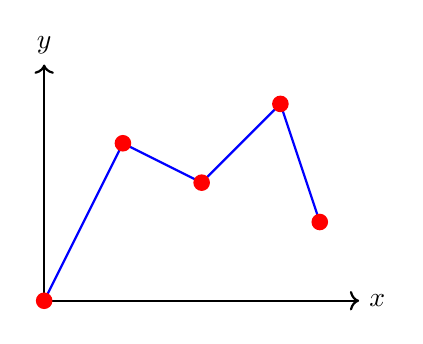
\begin{tikzpicture}
  \draw[thick, ->] (0,0) -- (4,0) node[right] {$x$};
  \draw[thick, ->] (0,0) -- (0,3) node[above] {$y$};
  \draw[blue, thick] (0,0) -- (1,2) -- (2,1.5) -- (3,2.5) -- (3.5,1);
  \foreach \x/\y in {0/0, 1/2, 2/1.5, 3/2.5, 3.5/1} {
    \fill[red] (\x,\y) circle (3pt);
  }
\end{tikzpicture}
\caption{Exemplo de figura em apêndice.}\label{FD}
\end{figure}


% Anexos
\annex
\chapter{Exemplo de um Primeiro Anexo} %opcional
\input{AneA/anexoA}

% Glossario
%\itaglossary
%\printglossary

% Folha de Registro do Documento
% Valores dos campos do formulario
\FRDitadata{\today} % Data de publicação (automática ou preencher manualmente)
\FRDitadocnro{DCTA/ITA/\itadoccode-000/2026} % Solicitar número à biblioteca
\FRDitaorgaointerno{Instituto Tecnológico de Aeronáutica -- ITA}
\FRDitapalavrasautor{Palavra1; Palavra2; Palavra3} % Palavras-chave sugeridas pelo autor
\FRDitapalavrasresult{Palavra1; Palavra2; Palavra3} % Palavras-chave resultantes da indexação
%Exemplo no caso de graduação (TG):
%\FRDitapalavraapresentacao{Trabalho de Graduação, ITA, São José dos Campos, 2015. \NumPenultimaPagina\ páginas.}
%Exemplo no caso de pós-graduação (msc, dsc):
\FRDitapalavraapresentacao{ITA, São José dos Campos. Curso de Mestrado. Programa de Pós-Graduação em Engenharia Aeronáutica e Mecânica. Área de Concentração. Orientador: Prof.~Dr. Nome do Orientador. Coorientadora: Prof$^\textnormal{a}$.~Dr$^\textnormal{a}$. Nome da Coorientadora. Defesa em DD/MM/AAAA. Publicada em DD/MM/AAAA.}
\FRDitaresumo{\placeholder{Inserir aqui o resumo em português. O resumo deve apresentar de forma concisa o objetivo, a metodologia, os resultados e as conclusões do trabalho. Deve ser redigido em parágrafo único, sem recuo na primeira linha, com espaçamento simples entre linhas. O resumo não deve ultrapassar 500 palavras para dissertações e teses, ou 250 palavras para trabalhos de graduação.}
}
%  Primeiro Parametro: Nacional ou Internacional -- N/I
%  Segundo parametro: Ostensivo, Reservado, Confidencial ou Secreto -- O/R/C/S
\FRDitaOpcoes{N}{O}
% Cria o formulario
\itaFRD

\end{document}
% Fim do Documento. O massacre acabou!!! :-)
